\documentclass[main.tex]{subfiles}

\begin{document}
	
	\begingroup
	
	\renewcommand{\cleardoublepage}{}
	
	\renewcommand{\clearpage}{}
	
	\chapter{Storing Groceries Task Overview}
	
	\chapterauthor{Torge Olliges, Tom-Eric Lehmkuhl, Evan Kapitzke, Jeremias Thun, Jan Neumann}

	\section{Goal}
	The goal of the Storing Groceries task is, like the name indicates, to store several groceries at their designated position. For the RoboCup this task has been simplified. The objects are all on a table and need to be sorted into a predefined shelf. The sorting has to be done by categories which need to be comprehensible by a human. This can be based on color, form or other categories. To fulfill this task the HSR has to identify the objects on the table and existing objects in the shelf. Furthermore it needs to grasp and place one object after the other. It also needs to navigate between the shelf and table. For additional points the HSR has to open doors. Overall the HSR has only 5 minutes to complete the task. 

	\section{Tasks}
	The figures \ref{grocery_seq_01} and \ref{grocery_seq_02} show the procedure of Storing Groceries. The following subsections explain the execution and procedure in detail and give insights into the decisions made resulting in the exact plan depicted below. Additionally a more in depth explanation of some of the challenges will be given.
	
		\begin{figure}[H]
			\centering
			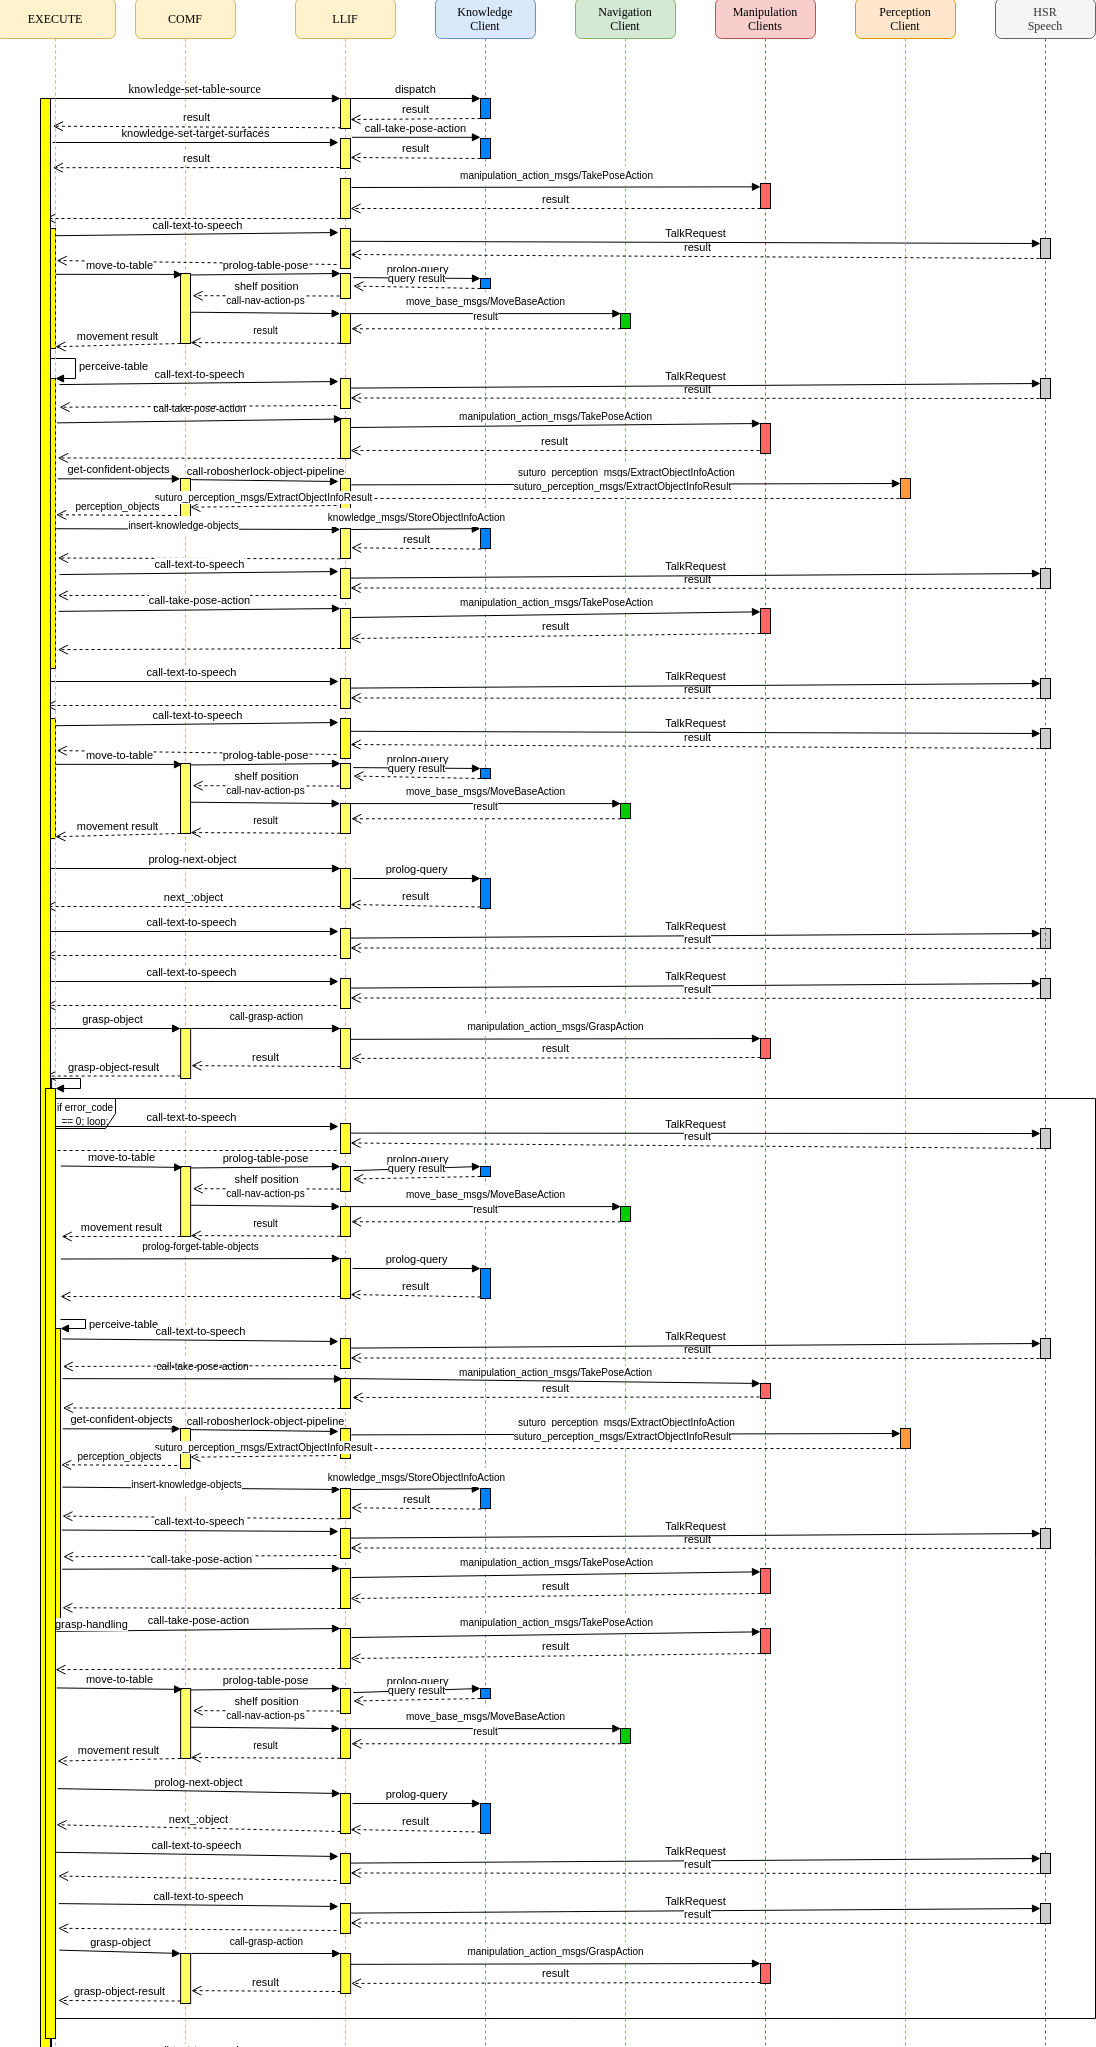
\includegraphics[width=0.85\textwidth]{pictures/diagramms/first-part-grocery-sequence.png}
			\caption{Sequence diagram of the complete run of the grocery storing task \textit{(explanations below)}}
			\label{grocery_seq_01}
		\end{figure}
		\begin{figure}[H]
			\centering
			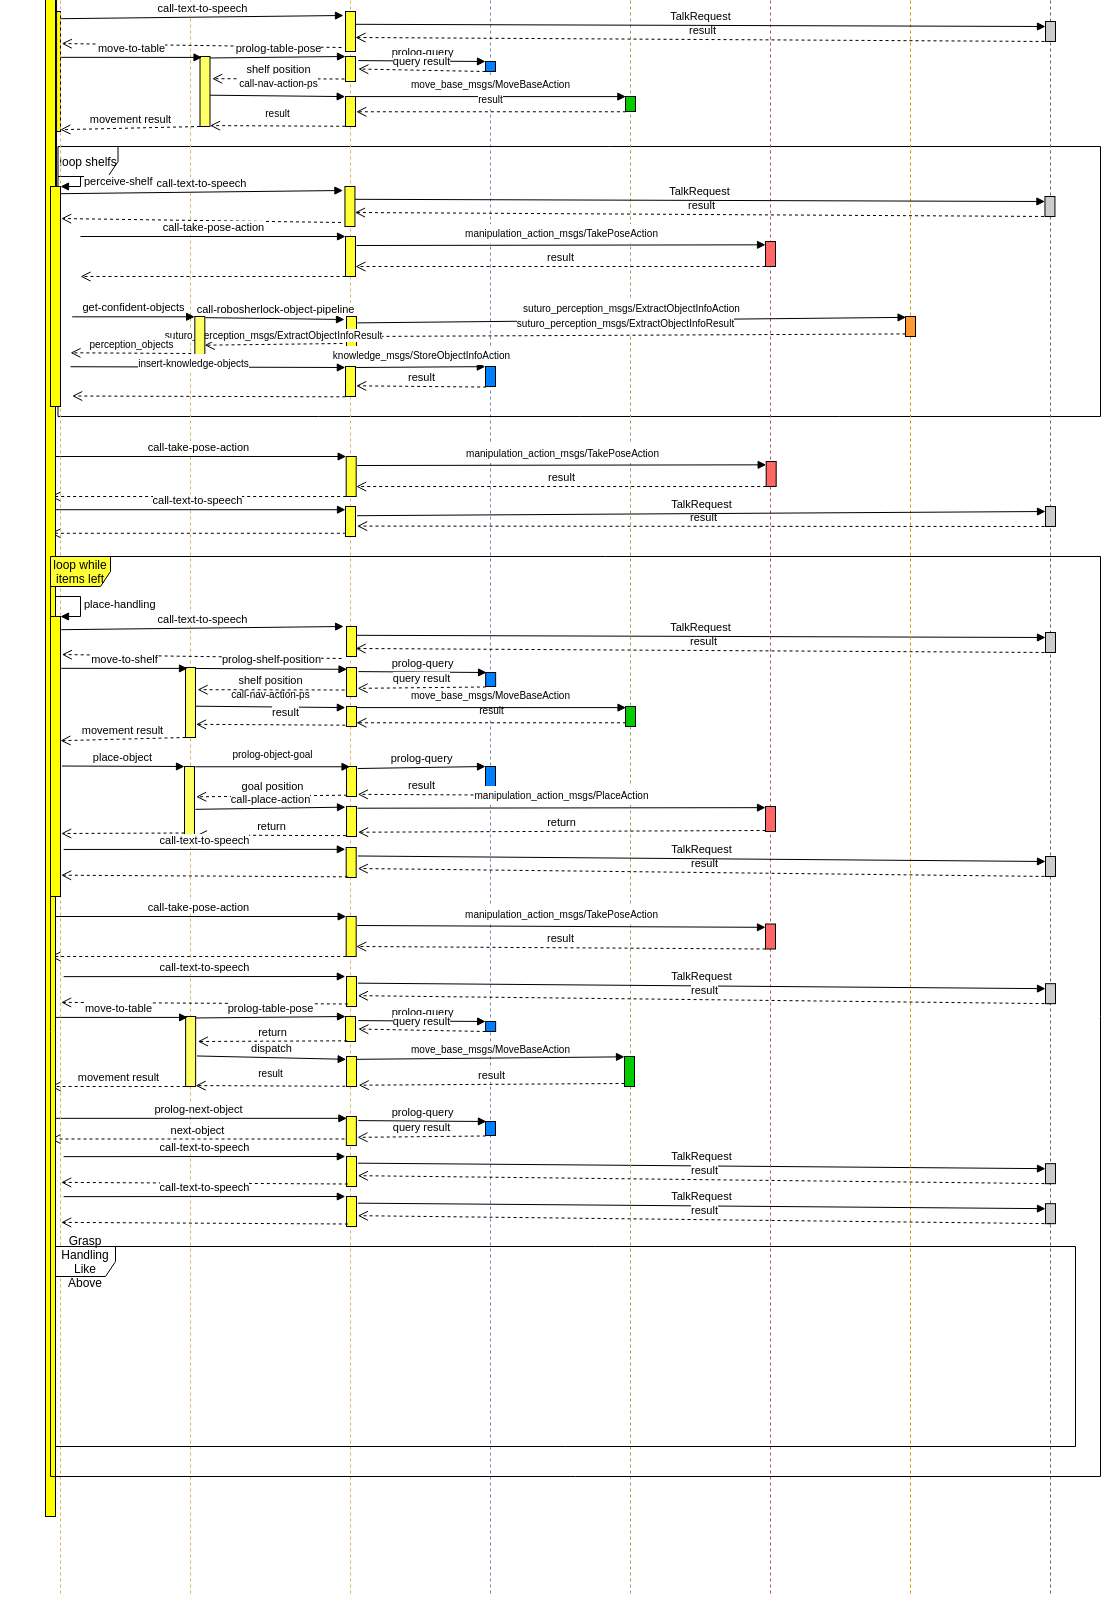
\includegraphics[width=0.85\textwidth]{pictures/diagramms/second-part-grocery-sequence.png}
			\caption{Sequence diagram of the complete run of the grocery storing task \textit{(explanations below)}}
			\label{grocery_seq_02}
		\end{figure}
		\textit{The sequence diagram in figure \ref{grocery_seq_01} and \ref{grocery_seq_01} does not depict when the action servers are running it rather displays the time they are actively used.}
	
	\subsection{Setup}
	

	% Knowledge: set-tables-source 
	According to the task only one table serves as the \texttt{source} for objects. In Knowledge it is allowed to set multiple \texttt{sources} for objects in order to allow greater compatibility and easier adaption to other tasks. For the current task at hand only the corresponding table is set as \texttt{source}. The same principle applies to the shelf which is set as \texttt{target} surface. Every surface e.g. tables, shelf's or the floor can be set as \texttt{source} or \texttt{target}.
	
	\subsection{Scan Table}
	
	% Manipulation: take pose action
	\begin{manipulation}
	The robot is set to the default pose to make sure it is in a neutral state. This is important in order to avoid moving the robot for example with an extended arm. Manipulation allows the use of predefined poses as well as setting a pose by defining the joint states. These joint states are then forwarded to \textit{Giskard}.\end{manipulation}
	
	% NLP: Talk Request
	\begin{nlp}
	To inform the developer as well as the people following the robot or evaluating it's behavior about what the robot is about to do, the robot will talk about it's actions. These talk requests are also used for safety measures so the robot can warn when it is going to move so bystanders can step aside. \end{nlp}
	
	% Knowledge: get table-poses
	\begin{knowledge}
	To start the task, Knowledge finds all the tables available, sorts them by their distance to the robot and then returns the list of their position to Planning, so that Planning can determine where the robot has to go first.\end{knowledge}
	
	% Navigation: moveBaseAction
	\begin{navigation}
	Planning determines a goal for the \texttt{move base action}. In this goal the HSR is turned $90^\circ$ to the nearest table, allowing it to look over it's shoulder having a clear view of the table without the arm in it's way. The default navigation client of the HSR then executes the action. \end{navigation}
	
	% NLP
	\begin{nlp}
	The robot then says that it is starting to perceive the table.\end{nlp}
	
	% Manipuilation: TakePoseAction
	\begin{manipulation}
	Manipulation gets the task to put the HSR into a pose to perceive an object depending on the height of the plane the object is on.
    That is necessary for Perception to get a good angle and distance to the object and to avoid having the robots arm block the cameras view.
    \end{manipulation}
	
	% Perception: Percieve and return data
	\begin{perception}
	The HSR takes a picture of the scene it is currently looking at and processes it with RoboSherlock. Based on the requested region the input images are filtered. The results i.e. the data of the perceived objects are then published by the \textit{perception\_actionserver} so planning can find them.\end{perception}
	
	% Knowledge: Store Data
	\begin{knowledge}
	Knowledge verifies the data of the objects, that were perceived and are supposed to be stored. If the class of an object is unknown to Knowledge or if it could not have been perceived with a high enough confidence, it is set to the class \texttt{Other}, if the dimensions are too small to actually be an object, it is rejected and so on. If the data for the given object is valid, the object gets added to the Knowledge base. Should the objects stand close to one another, they get organized in a group. Groups are used to sort objects and can be used to determine if an object is hard to grasp.
	\end{knowledge}
	% NLP: Talk Request
	
	% Manipulation: Take pose
	\begin{manipulation}
	In order to grasp an object the HSR needs to look straight at the object with it's base. Therefore the HSR needs to be in it's default pose allowing safe movement.
	\end{manipulation}
	% 2x NLP: Talk
	
	% Knowledge: prolog_ table_pose
	\begin{knowledge}
	For Planning to give the orders to move the robot to the table with the object to grasp on it, Knowledge once again provides the position data of the nearest table.
	\end{knowledge}
	
	% Navigation: MoveBaseAction
	\begin{navigation}
	Turn the HSR by $90^\circ$ so it looks straight at the table and can grasp an object.
	\end{navigation}
	
	\subsection{Grasp Object}
	
	\label{grasp-object}
	% Knowledge: next_object
	\begin{knowledge}
	The Knowledge base now determines which object should be grasped next, to place it in one of the shelves. This decision is purely based on the distance of the objects to the robot so that the nearest object standing on any of the tables will be taken first.
	\end{knowledge}
	
	% 2x NLP: Talk Request
	\begin{nlp}
	The HSR says which object will be grasped. The object name is the object identifier without the unique string prefix for the knowledge base.
	\end{nlp}
	
	% Manipulation: GraspAction
	\begin{manipulation}
	Manipulation gets the task to grasp the given object. Different modes of grasping are possible but at the moment only frontal grasping is used actively. At first the orientation of the gripper is calculated based on the HSR's rotation. Additionally the collision for the object to grasp gets deactivated. This is important since otherwise \textit{Giskard} would stop the gripper in front of the object. During the course of the project it became apparent that \textit{Giskard} had some difficulties planning the movement of the gripper inside of shelves. Therefore an additional way point is calculated which ensures the gripper can move in a straight line in and out of a shelf. After the gripper is closed around the object a check is started to probe whether the object is in the gripper. If successful the object gets attached to the gripper to ensure it's taken into account for future motion planning.   
	\end{manipulation}
	
	% Planning: 
	\begin{planning}
	This whole thing is gonna be looped % todo
	\end{planning}
	
	% NLP
	
	% Knowledge: Shelf Positions
	\begin{knowledge}
	Knowledge finds all the shelves available and sorts them, just like the tables before, by their distance to the robot. This way, the Robot can navigate to all the shelves starting with the nearest one to scan the objects already in place.
	\end{knowledge}
	
	% Navigation: Move to Shelf
	\begin{navigation}
	% todo
	\end{navigation}
	
	\subsection{Scan shelf floors}
	
	% Planning: Loop through all shelf floors
	\begin{planning}
	In the scan shelf floors function % todo
	\end{planning}
	% NLP
	\begin{nlp}
	The robot informs which shelf he is currently looking at. The robot scans the shelf from the bottom up from shelf 0 to shelf 2.\end{nlp}
	
	% Manipulation: go into percieve pose
	\begin{manipulation}
	Since the shelf floors are of different heights the HSR has to take multiple perceive poses.
	\end{manipulation}
	
	% Perception: Percieve shelf
	\begin{perception}
	The HSR takes a picture of the shelf it is currently looking at and processes it with \textit{RoboSherlock}. Based on the requested shelf level the input images are filtered in order to perceive only objects in one specific level. The results are then published by the \textit{perception\_actionserver}.
	\end{perception}
	
	% Knowledge: Store new Objects
	\begin{knowledge}
	Knowledge checks the data of the objects, that are supposed to be stored. If the class of an object is unknown to Knowledge, it is set to other. If the data for the given object is valid, the object gets added to the Knowledge base. Should other objects be close to the new one, they get organized in a group. Groups are used to sort objects and can be used to determine if an object is hard to grasp.
	\end{knowledge}
	
	\subsection{Place Object}
	
	% Planning: Loop this while some items are left
	\begin{planning}
	The following part is executed until either all objects are handled, the HSR can not find any other objects or the HSR is told via NLP commands to stop it's current behavior.
	\end{planning}
	
	% Knowledge: shelf positions
	\begin{knowledge}
	Knowledge again provides a list of all the shelf surfaces, sorted by their distance to the robot and returns it to Planning.
	\end{knowledge}
	
	% navigation: move to shelf
	\begin{navigation}
	The HSR moves to the shelf so it can place the object currently in the gripper.
	\end{navigation}
	
	% Knowledge: Object goal pose
	\begin{knowledge}
	Knowledge now determines the most suitable position for the object which is currently handled. The way this decision is made is explained in the Knowledge function documentation \ref{sec:kn_find_surf}. For now it is enough to know, that Knowledge finds a suitable surface for that object and the exact coordinates in the world frame based on the objects properties and all other known objects in the scene.
	\end{knowledge}
	
	% Manipulation: PlaceAction
	\begin{manipulation}
	The procedure of placing an object is very similar to the grasping process. Different modes are available but only the grasp from front mode is actively used. The orientation of the gripper is calculated based on the HSR's rotation and a way point is determined to allow smooth in and  out movement for shelves. After the object gets released from the gripper its collision is deactivated to avoid problems with the collision box of the gripper during the backwards movement. Afterwards collision for the object gets enabled again. The actual movement planning and execution is done by \textit{Giskard}.   	
	\end{manipulation}
	
	% NLP
	
	% Manipulation: TakePoseAction
	\begin{manipulation}
	The robot is set to the default pose. To avoid collisions.
	\end{manipulation}
	% NLP
	
	% Knowledge: table pose
	
	% Knowledge: next_object
	\begin{knowledge}
	Then, Knowledge again finds the nearest object standing on a table that should be handled next.
	\end{knowledge}
	
	% 2x NLP
	\begin{manipulation}
	Grasping the object is once again executed as described under \ref{grasp-object}.
	\end{manipulation}
	
	% Planning: Finish
	\begin{planning}
	If no objects have to be handled the robot stops.
	\end{planning}
	
	
	\section{Conclusion}

	The outcome of Storing Groceries can be declared as successful. It has been tested on multiple occasions; like the simulated RoboCup, the demonstrations of the second and the third milestone. 
	Even though there have been minor setbacks like failing to grasp objects on the first try this lead to showcasing the failure handling capabilities.
	There have also been problems which were caused by hardware issues like the movement of the robot which failed because of the magnet sensors or the problem of \textit{Giskard} avoiding collision with the shelf in the simulation which was seen in the third milestone demo.
	These Problems do not implicate that the plan wasn't working it just had some low level problems and would have performed the tasks successfully otherwise.
	
	
	\endgroup
	
\end{document}
